\lstset{language=HMMLanguage,numbers=left,breaklines=true,numbersep=0pt}
\subsection{Sensors}
\begin{frame}
	\frametitle{Sensors}
	\begin{itemize}
		\item We choose the following sensors, to have a diversity of information about the problem domain:
		\begin{itemize}
		  \item PIR - presence of a moving person
		  \item Ultrasonic - distance a person or object, presence of a particular spot
		  \item Photoresistor - Light intensity of a room
		\end{itemize}
		\item These sensors are cheap and accessible
		\item In order to gain knowledge on how to use each sensor and their limitations, we conclude some tests
		\begin{itemize}
		  \item Precision
		  \item Effective distance
		  \item Latency
		\end{itemize}
	\end{itemize}
\end{frame}
\subsubsection{PIR}
\begin{frame}
  \frametitle{PIR}
  What we did to improve our results:
	\begin{itemize}
	  \item Probe the sensor a couple of times
	  \item Average over the probes
	  \item If average is above some threshold then report presence of a moving person
	\end{itemize}
Effect: Increases the time it takes to get a result from the sensor, but the amount of time negligible in the context of the whole systems running time
    %We probed the output a couple of times and averaging over them to remove noise, this on the otherhand worsened of response time of our system but in the system of a whole this difference is neglible.
\end{frame}
\subsubsection{Ultrasonic}
\begin{frame}
	\frametitle{Ultrasonic}
	No improvements were needed for this sensor, but if more precise result were required by the use case.
	The implementation should also account for:
	\begin{itemize}
    \item Temperature of the room - a sensor for measuring temperature, would be required
    \item Dobbler effect for moving target - requires knowledge about velocity and direction
	\end{itemize}
\end{frame}
\begin{frame}[fragile]
	\frametitle{Ultrasonic code example}
	\begin{lstlisting}   
  unsigned long Ultrasonic::measureTiming(){
    digitalWrite(trigPin, LOW);   // Ensure low
    delayMicroseconds(2);         // Wait for stable low
    digitalWrite(trigPin, HIGH);  // Set trigger pin to high for 10 microseconds
    delayMicroseconds(10);        // to initiate sensor cycle

    digitalWrite(trigPin, LOW);   // Then set low again, the sensor will now emit and receive
                                  // 8 cycles of ultrasonic sound waves at 40 khz

    return pulseIn(echoPin,HIGH); // Now wait for the sensor to output a pulse,
                                  // the pulse width corresponds to a distance,
                                  // given delta t from send to recieved.
  }
  
  unsigned long Ultrasonic::getDistance(){
    return measureTiming()/58;    // 58 approximates (speedOfSound*measureTiming())/2
  }
	\end{lstlisting}
\end{frame}
\subsection{Actuators}
\begin{frame}
	\frametitle{Actuators}
	%in the report we have not really touched on any implementation of actuator.
	An actuator in our system could be:
	\begin{itemize}
		\item A SPDT relay - but this would require some rewiring and a SPDT switch too, which is not preferred
		\item The embedded subsystem system being an intermediate switch in the wall plug
		\begin{figure}[htbp]
		    \centering
        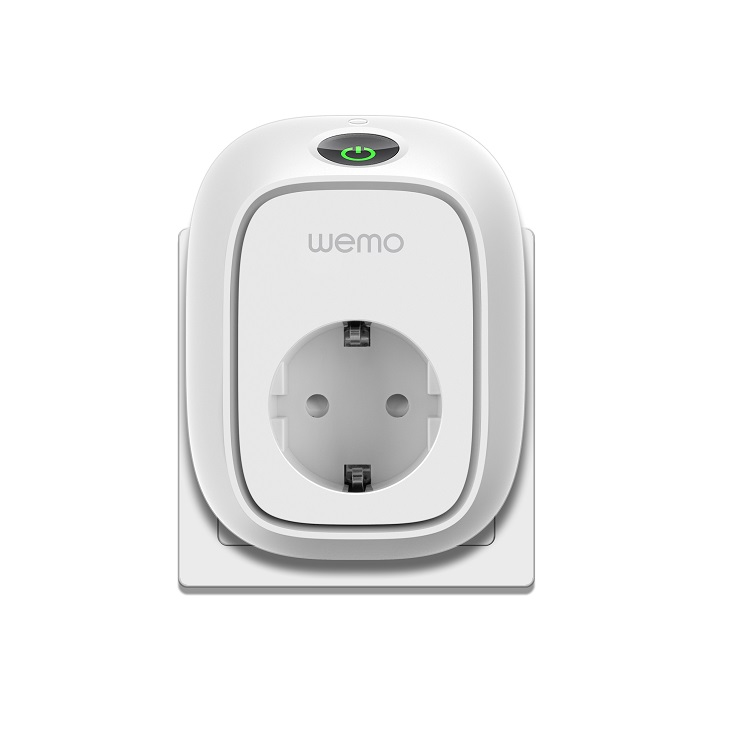
\includegraphics[width=\textwidth/2]{Images/wemo.jpeg}
		\end{figure}
	\end{itemize}
\end{frame}
